\documentclass[a4paper, 10pt, french]{article}
% Préambule; packages qui peuvent être utiles
   \RequirePackage[T1]{fontenc}        % Ce package pourrit les pdf...
   \RequirePackage{babel,indentfirst}  % Pour les césures correctes,
                                       % et pour indenter au début de chaque paragraphe
   \RequirePackage[utf8]{inputenc}   % Pour pouvoir utiliser directement les accents
                                     % et autres caractères français
   % \RequirePackage{lmodern,tgpagella} % Police de caractères
   \textwidth 17cm \textheight 25cm \oddsidemargin -0.24cm % Définition taille de la page
   \evensidemargin -1.24cm \topskip 0cm \headheight -1.5cm % Définition des marges
   \RequirePackage{latexsym}                  % Symboles
   \RequirePackage{amsmath}                   % Symboles mathématiques
   \RequirePackage{tikz}   % Pour faire des schémas
   \RequirePackage{graphicx} % Pour inclure des images
   \RequirePackage{listings} % pour mettre des listings
% Fin Préambule; package qui peuvent être utiles

\title{ \bf Rapport de TP AOD}
\author{
CATHRINE Damien ~ SAINRAT Paul
\\ Equipe 19
}

\begin{document}

\maketitle

%%%%%%%%%%%%%%%%%%%%%%%%%%%%%%%%%%%%%%%%%%%%%%
\section{Equation de Bellman}
\paragraph{Analyse} Nous devons démontrer qu'un sous-arbre d'un arbre optimal est lui même optimal. Intéressons nous à un arbre $A$ triant l'ensemble $E = \{e_0,e_1,...,e_{n-1}\}$ avec $e_0<e_1<.....<e_{n-1}$. Soit $a$ un sous-arbre non optimal de $A$ tel que $a$ trie un sous ensemble F de E. Nous allons donc déterminer si l'arbre A est optimal :
\[\sum_{e_i\in E} p_i \times \Delta_{A}(e_i) \]
On peut scinder cette somme en deux en séparant les élément de $F$ et de $E/F$
\[\sum_{e_i\in F} p_i \times \Delta_{A}(e_i) + \sum_{e_i\in E/F} p_i \times \Delta_{A}(e_i) \]
On remarque que la somme de gauche n'est pas minimale dans l'ensemble des arbres triant les éléments de F car a n'est pas un arbre optimal. En conséquent la somme de départ elle même n'est pas minimal dans l'ensemble des arbres triant les éléments de E. Par définitions l'arbre A ne peut pas être optimal. Nous avons donc prouvé que si le sous arbre n'est pas optimal, alors l'arbre auquel il appartient ne peut pas être optimal. Ce qui implique que si un arbre est optimal alors tout sous-arbre de cet arbre l'est aussi.
\\
\\
Soit $C(noeud, \Delta_{A}(e))$ la profondeur moyenne, ou le nombre de comparaisons en moyenne pour accèder à un élément quelconque dans le sous-arbre de racine $noeud$ et de profondeur $\Delta_{A}(e)$ et soit $p$ la fréquence d'apparition de l'élément associé au noeud. Alors on a :

\[  C(noeud, \Delta_{A}(e)) = C(noeud.filsG, \Delta_{A}(e) + 1) + C(noeud.filsD, \Delta_{A}(e) + 1) + \Delta_{A}(e) \times p \]

Avec :

\[  C*(noeud, \Delta_{A}(e)) = min(C(noeud, \Delta_{A}(e))) \]

On obtient l'équation de Bellman suivante :

\[  C*(noeud, \Delta_{A}(e)) = C*(noeud.filsG, \Delta_{A}(e)+1) + C*(noeud.filsD, \Delta_{A}(e)+1) + \Delta_{A}(e) \times p \]

Si $noeud.filsG$ ou $noeud.filsG$ n'existe pas, Alors $\forall \Delta_{A}(e), C*(noeud.filsG/D, \Delta_{A}(e)) = 0$

\paragraph{Implémentation Naïve} Notre première implémentation à été d'essayer d'utiliser la formule de Bellman de manière assez naïve. Ainsi pour chaque élément d'un tableau donné, nous essayons cet élément comme racine : nous calcul alors le coût en moyenne de l'arbre généré à l'aide d'un appel de cette même fonction sur le tableau à gauche de cet élément et sur le tableau à droite de cet élément. Cet approche en plus d'être très coûteuse ne permet pas de récupérer les racines facilement. Elle n'utilise pas d'autre mémoire que la pile. La complexité pour n éléments $C(n)$ revient alors à :

\[ C(n) = n \times C(n-1) \]

Ce qui revient alors à $C(n) = O(n!)$

%%%%%%%%%%%%%%%%%%%%%%%%%%%%%%%%%%%%%%%%%%%%%%
\newpage
\section{Principe de notre  programme}
Nous utilisons 2 fonctions : une itérative {\tt explore\_and\_store} permettant de parcourir l'ensemble des arbres possible dans le dictionnaire donné et stockant le coût minimal et sa racine associée, assurant ainsi l'unicité du parcours de chaque sous-arbre. Et 1 récursive {\tt fill\_BST} permettant de remplir la structure de donnée spécialisée pour stocker l'arbre avant de l'afficher.

Nous commençons alors par les sous-arbres de 1 élément (qui correspondent aux fréquences du dictionnaire) puis ceux de 2 et ainsi de suite jusqu'à avoir l'unique arbre de longueur voulue. Chaque construction se servant des données des sous-arbres précédents pour générer le coût minimal et la racine correspondante.
Ces données sont stockées dans un tableau à 2 dimension, étant stocké de manière contiguë et optimale pour le parcours présenté précédemment. Ainsi on accède au coût du sous-arbre de longueur $L$ et commençant à l'indice $b$ dans le dictionnaire, dans le tableau des Coûts $T$ avec $T[L][b]$. Les arbres de longueur 1 sont stocké d'abord puis ceux de longueur 2 ... le tout de manière continue. Cela permet alors de limiter le nombre de défauts de cache. Les racines sont stockées dans une structure similaire composés d'entiers sur moins de bits (Les coûts sont stockés sur les {\tt long long}, et les racines sur des {\tt short}).

%%%%%%%%%%%%%%%%%%%%%%%%%%%%%%%%%%%%%%%%%%%%%%
\section{Analyse du coût théorique}
 Comme nous l'avons expliqué dans le paragraphe précèdent, notre fonction principale prend n éléments, calcule le coût des sous-arbres allant de 1 à n éléments. Et sélectionne parmi les arbres composés des mêmes éléments, celui de plus petit coût avant de le stocker dans un tableau ou il sera indicé par la taille de l'arbre et l'indice de l'élément le plus petit qui le constitue.



  \subsection{Nombre  d'opérations en pire cas}
     Notre programme itératif contient boucles 3 boucles, la première parcours toutes les tailles d'arbre possible, la seconde tout les arbres de la dite taille possible, et la dernière les élément qui composent le dit arbres. Ainsi, si on considère que les opérations qui s'effectuent dans la dernière boucle sont primaires et que leurs nombre est négligeables correspondant ici à $\alpha$, nous obtenons un nombre d'opérations correspondant à la somme suivante :
      $$C(n,\alpha) = \sum_{l=1}^{n} \sum_{k=0}^{n-l} \sum_{i=k}^{k+l} \alpha
                    = \sum_{l=1}^{n} \sum_{k=0}^{n-l} \alpha l
                    = \sum_{l=1}^{n} \alpha l (n-l+1)
                    = \alpha (n-1) \sum_{l=1}^{n} l - \sum_{l=1}^{n} l^2 $$
      $$C(n,\alpha) = \frac{\alpha n (n+1)^2}{2} - \frac{n(n+1)(2n+1)}{6}
                    = O(n^3)$$

  \subsection{Place mémoire requise}
 Lors de l'exécution de notre programme nous utilisons deux structures que nous avons créer que l'on peut identifier comme étant des tableau. Dans le premier nous stockons le coût des arbres de différentes tailles, pour indicer les éléments de ce tableau nous utilisons la taille de l'arbre pour les lignes, et l'indice de l'élément le plus petit parmi ceux qui constituent l'arbre pour les colonnes (cf: Figure \ref{fig:struct1}).



 En mémoire, toutes les valeurs sont stockée de façon contiguës, mais comme la quantité d'arbres possible varie d'une taille d'arbres à l'autre (Pour n élément, il y à (n-l) arbres de taille l). Nous utilisons donc un tableau à n case qui stocke des pointeur permettant d'accéder aux différentes ligne du premier tableau (cf : Figure\ref{fig:struct2}).



  La seconde structures est construites sur le même modèle que la première sauf que au lieu de stocker le coût des arbres, nous y stockons leur racines.

    Ainsi la mémoire utilisé par notre programme est essentiellement celle utilisée par nos 2 structures. Soit, pour traiter $n$ éléments nous utilisons un espace mémoire que nous pouvons décrire par la somme suivante :
    $$M(n) = 2 \times (n + \sum_{i=n}^{1} i) = 2 \times (n + \frac{n(n+1)}{2}) = O(n^2)$$

  \subsection{Nombre de défauts de cache sur le modèle CO}
    Étant donné que les données sont stockées consécutivement en mémoire cela limite le nombre de défauts de cache mais ils restent néanmoins nombreux. En effet dans le pire des cas chaque calcul de coût d'un sous-arbre peut aller chercher 2 coûts précédemment calculés qui peuvent se trouver sur deux lignes du tableaux différentes, les données peuvent potentiellement ne pas être dans le cache et le chargement dans le cache d'une des deux données peut provoquer un défaut de cache sur la deuxième  : \\
    Soit L la longueur d'une ligne de cache et n le nombre d'élément dans le dictionnaire :
     $$D(n) = 2 \times (\frac{n}{L} + \frac{2}{L} \sum_{i=n}^{1} i^2)
            = \frac{2n}{L} + \frac{n(n+1)(2n+1)}{3L}
            = O(\frac{n^3}{L})$$




%%%%%%%%%%%%%%%%%%%%%%%%%%%%%%%%%%%%%%%%%%%%%%


\section{Compte rendu d'expérimentation}
  \subsection{Conditions expérimentales}
    \subsubsection{Description synthétique de la machine}
      Les test ont été fait sur un ordinateur portable ayant comme CPU : {\tt Intel(R) Core(TM) i7-4700MQ CPU @ 2.40GHz}, 16 GB de RAM et sur un Ubuntu, la machine étant monopolisée pour les tests.

    \subsubsection{Méthode utilisée pour les mesures de temps}
      Les mesures de temps ont été faites l'une après l'autre en utilisant la fonction {\tt time}, le même test étant fait 5 fois de suite.

  \subsection{Mesures expérimentales}
    \begin{figure}[h]
      \begin{center}
        \begin{tabular}{|l||r||r|r|r||}
          \hline
          \hline
                        & temps      & temps       & temps \\
                        & min        & max         & moyen \\
          \hline
          \hline
            benchmark1 & $1\mu s$    & $2\mu s$    & $1.8\mu s$  \\
          \hline
            benchmark2 & $1\mu s$    & $2\mu s$    & $1.6\mu s$  \\
          \hline
            benchmark3 & $1.873 s$   & $1.976 s$   & $1.912 s$   \\
          \hline
            benchmark4 & $23.921 s$  & $25.099 s$  & $24.417 s$  \\
          \hline
            benchmark5 &$1min31.478s$&$1min36.227s$&$1min33.923s$\\
          \hline
            benchmark6 &$7min30.823s$&$7min52.132s$&$7min39.404s$\\
          \hline
          \hline
        \end{tabular}
        \caption{Mesures des temps minimum, maximum et moyen de 5 exécutions pour les 6 benchmarks.}
        \label{table-temps}
      \end{center}
    \end{figure}

\subsection{Analyse des résultats expérimentaux}
    En considérant que le coût temporel de notre programme est en $O(n^3)$ et en prenant par exemple le benchmark 6 qui contient 5000 éléments et en considérant que pour chaque éléments on a une dizaines de cycles d'horloge du CPU qui sont occupés, cela donne un peu moins de la dizaine de minute en ordre de grandeur ce qui est parfaitement cohérent. ($NbSec = 10 \times 5000^3 \times 2.4 \times 10^{-9}$).

    Malgré une amélioration du temps nécessaire pour calculer un arbre optimal par rapport à notre premier programme récursif, nous constatons tout de même que le temps nécessaire pour calculer un arbre avec de nombreux éléments reste important. Nous avons remarqué que les calculs des coût des arbres d'une même ligne était indépendant, nous pensons donc qu'il est possible d'optimiser le temps de calcul du programme en parallélisant les calcul de coût qui s'effectue sur une même ligne du tableau.

    Nous avons remarqué que pour le benchmark3 qui contient de gros entiers (proche du million pour certains), le type {\tt unsigned long} ne semblait pas suffire pour calculer le coût total. Nous avons alors utilisé le type {\tt long long}. Mais cela rend l'affichage de ce coût négatif même en utilisant le bon spécificateur de format ({\tt \%lld}) ce qui reste assez étrange.



    \begin{figure}[p]
  \caption{Structure de stockage}
  \centering
  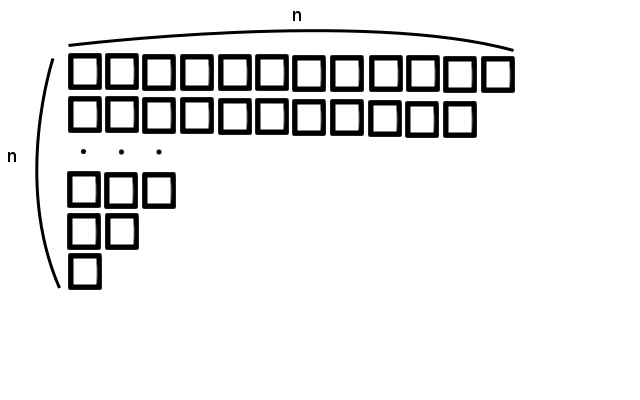
\includegraphics[scale=0.45]{struct1}
  \label{fig:struct1}
\end{figure}

      \begin{figure}[p]
  \caption{Structure de stockage}
  \centering
  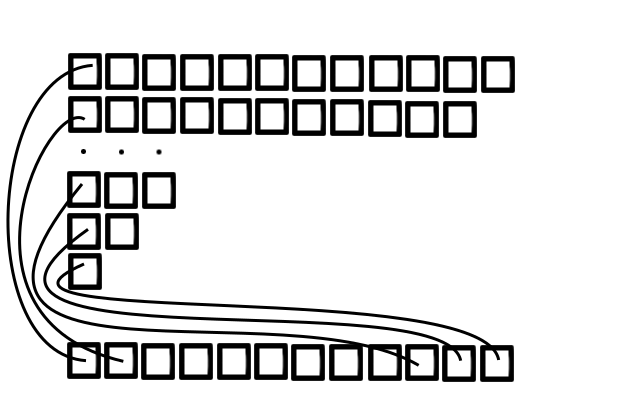
\includegraphics[scale=0.45]{struct2}
  \label{fig:struct2}
\end{figure}




\end{document}
%% Fin mise au format
